\section{QR-Codes}\label{chap:qrcodes}
Dieses Kapitel dreht sich um QR-Codes. Es enthält allgemeine Informationen sowie eine Beschreibung, wie Nutzdaten auf einen QR-Code codiert beziehungsweise aus ihm decodiert werden.

\subsection{Allgemeines}
Wie bereits in Kapitel~\ref{chap:history} und \ref{chap:overview} erwähnt, wurde der QR-Code 1994 von der japanischen Firma \textit{DENSO Corporation} (gegründet 1949 als \textit{Nippondenso Co. Ltd.}) entwickelt. Wie der ausgeschriebene Name \textbf{Q}uick \textbf{R}esponse (schnelle Antwort) erwarten lässt, zeichnet sich der QR-Code vor allem durch die sehr schnelle Lesbarkeit aus. Diese ist in dem markanten Suchmuster des Codes begründet, welches gleichzeitig auch zur Lageerkennung verwendet wird.
Nachdem die Grundidee 1994 entwickelt worden war, wurde sie 1997 verbessert und im selben Jahr in der AIM\footnote{Automatic Identification and Mobility} Spezifikation ISS 97-001 beschrieben. Diese Spezifikation ist heute unter dem Namen QR-Code Model 1 bekannt. Ihr Hauptmerkmal ist eine immer schwarz gefärbte Zelle in der Ecke unten rechts, die von drei weißen Zellen umgeben ist (siehe Abbildung~\ref{fig:qrModel1}).\\
Im Jahr 2000 wurde dann eine überarbeitete Version des Codes in der ISO/IEC\footnote{International Organization for Standardization/International Electrotechnical Commission} Norm 18004:2000 beschrieben. Diese wurde umgangssprachlich als QR-Code Model 2 bezeichnet. Im Vergleich zu Model 1 besitzt das Model 2 die sechsfache Datenkapazität. Zudem wurden weitere Orientierungsmuster hinzugefügt, welche \zitext{wie kleine Suchmuster zur Ausrichtung des Referenzgitters im Code strukturiert verteilt sind.}{\cite{Lenk2012}}\\
\begin{figure}[htbp]
	\parbox{.47\textwidth}
	{
		\centering
		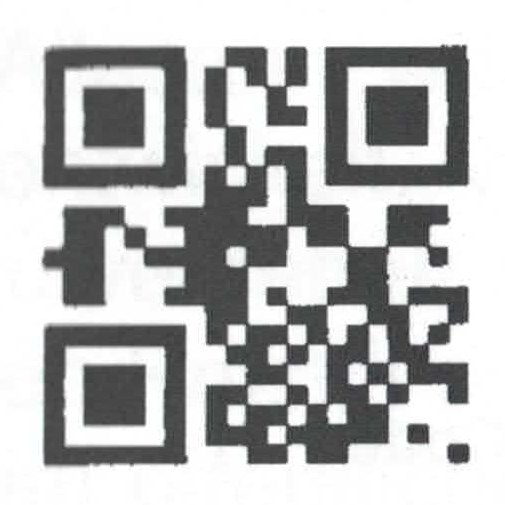
\includegraphics[height=2.5cm]{Bilder/QR_Code_Model_1.png}
		\caption[QR-Code Model 1]{QR-Code Model 1\footnotemark}
		\label{fig:qrModel1}
	}
	\hfill
	\parbox{.47\textwidth}
	{
		\centering
		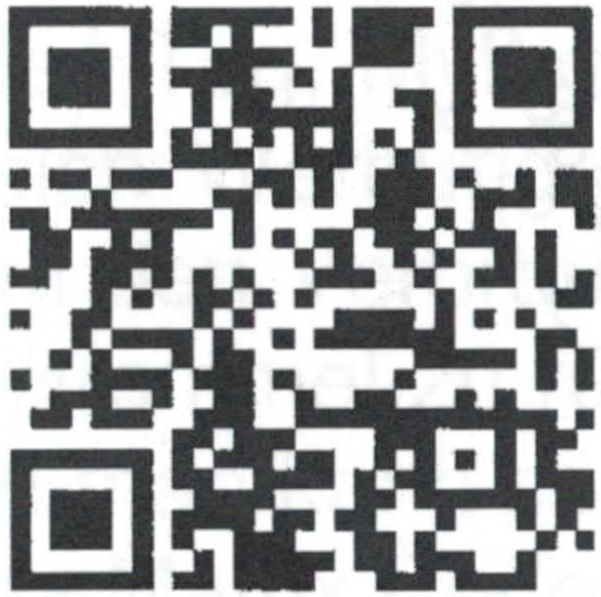
\includegraphics[height=2.5cm]{Bilder/QR_Code_Model_2.png}
		\caption[QR-Code Model 2]{QR-Code Model 2\textsuperscript{\ref{ftn:second}}}
		\label{fig:qrModel2}
	}
	\hfill
\end{figure}
\footnotetext{Quelle: \cite[3]{Lenk2012}\label{ftn:second}}~\\
Die heute verwendete Form des QR-Codes ist eine verbesserte Form des Model 2. 
Sie wurde 2006 in der Norm ISO/IEC 18004:2006 beschrieben und wird normalerweise als QR-Code 2005 (siehe Abbildung~\ref{fig:qr2005}) bezeichnet. 
2009 wurde sie um einige Detailverbesserungen ergänzt. 
In dieser Norm (18004:2006) wurde der normale QR-Code um den Micro QR-Code und den GS1 QR-Code erweitert. \pagebreak
Im weiteren Verlauf dieses Kapitels wird der QR-Code 2005 als Grundlage für alle weiteren Erläuterungen verwendet.

\begin{figure}[htbp]
	\centering
	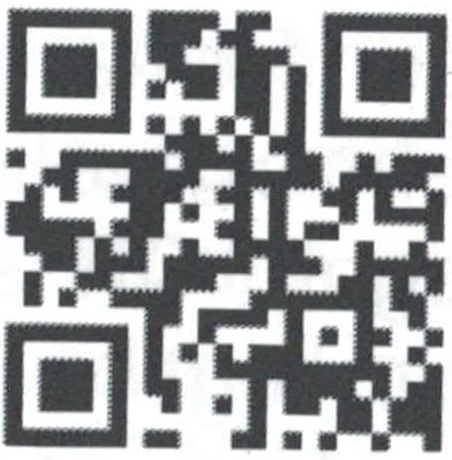
\includegraphics[width=2.5cm]{Bilder/QR_Code_2005.png}
	\caption[QR-Code 2005]{QR-Code 2005\footnotemark}
	\label{fig:qr2005}
	\hfill
\end{figure}
\footnotetext{Quelle: \cite[4]{Lenk2012}}

\subsection{Daten codieren}
Wie aber wird nun ein Text, eine Nummer oder auch eine URL in einem QR-Code codiert? Bevor dieser Prozess genauer beleuchtet wird, soll kurz die \glqq Anatomie\grqq~eines QR-Codes vorgestellt werden. In Abbildung~\ref{fig:qranatomy} sind die wichtigsten visuellen Merkmale eines Codes farbig hervorgehoben worden. Das rote Quadrat, welches der Grundbaustein des QR-Codes ist, nennt man Modul. Insgesamt besitzt der Code eine quadratische Matrixstruktur mit hellen und dunklen Modulen, welche jeweils ein Bit repräsentieren. Die Matrix ist immer ungerade und bewegt sich im Bereich von 21 x 21 bis 177 x 177. Insgesamt gibt es 40 verschiedene Matrix-Versionen (1 bis 40), die von einer zur nächsten um jeweils 4 Zellen an jeder Seite erweitert wird.\\
Die großen, grün hervorgehobenen Vierecke in den drei Ecken nennt man Suchmuster. Sie dienen zum schnellen Auffinden des Codes im Leseprozess. Drei Ecken deshalb, um eine Eindeutigkeit des omnidirektional lesbaren Codes zu garantieren. Zudem lassen sich durch die Quadrate auch Verzerrungen des Codes erkennen. Der Rahmen des inneren Quadrates ist genau so breit wie ein Modul. Das innere Quadrat besitzt die Breite 3 x 3 Module. 

\begin{figure}[htbp]
	\centering
	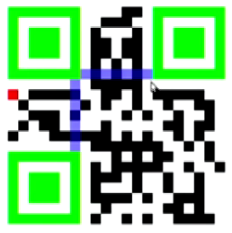
\includegraphics[width=5cm]{Bilder/QR_Code_Anatomie.png}
	\caption[Anatomie eines QR-Codes]{Anatomie eines QR-Codes\footnotemark}
	\label{fig:qranatomy}
	\hfill
\end{figure}
\footnotetext{Quelle: \cite{Plotz2015}}

Die blau hinterlegten Zellen markieren die sogenannten Taktzellen. Diese zeigen dem Scanner an, wie groß die Matrix ist. Die Taktzellen sind immer abwechselnd weiß und schwarz.
Weiterhin enthalten alle QR-Codes ab der Größe 25 x 25 eine oder (je nach Größe) mehrere Orientierungszellen, wie sie in Abbildung~\ref{fig:qrorientation} in Violett hervorgehoben ist.
Diese Orientierungszellen helfen dem Scanner in den größeren Codes, vor allem in verzerrten Codes die einzelnen Zellen bewerten zu können.
\begin{figure}[htbp]
	\centering
	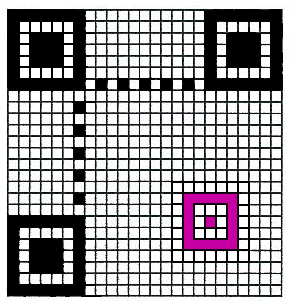
\includegraphics[width=5cm]{Bilder/Orientierungszelle.png}
	\caption[QR-Code mit Orientierungszelle]{QR-Code mit Orientierungszelle\footnotemark}
	\label{fig:qrorientation}
	%\hfill
\end{figure}
\footnotetext{Quelle: \cite[100]{Lenk2012}}~\\
Möchte man nun Daten codieren, so spezifiziert die ISO-Norm einen Ablauf, der in den folgenden Unterpunkten beschriebenen wird:\\
\vspace*{-0.8cm}
\subsubsection*{1. Datenanalyse}
Zuerst wird entschieden, welcher Kodiermodus verwendet wird. Es gibt vier verschiedene Modi, die hauptsächlich im Einsatz sind: 
\begin{itemize}
	\item \textbf{Numerisch}. Dieser Modus umfasst die Zeichen  0, 1, \dots, 9. \\
	In diesem Modus werden immer 3 Zeichen von links nach rechts zusammengefasst und in 10 Bit codiert. Bei einem Rest von 2 beziehungsweise einem Zeichen werden diese in 7 Bit beziehungsweise 4 Bit codiert. So wird zum Beispiel die Ziffernfolge "01234567"{} in 012 345 67 aufgeteilt. Der Numerikmodus wird mit der Kennung 0001 erkannt.
	\item \textbf{Alphanumerisch}. Dieser Modus erkennt die in Tabelle~\ref{tab:refalphanum} im Anhang dargestellten Zeichen und codiert immer zwei von ihnen in 11 Bit. Die Kennung dieses Modus ist 0010.
	\item \textbf{Byte}. Der Byte-Modus akzeptiert alle ISO-Zeichen nach ISO-8859-1:1988 (Latin)  oder auch andere Zeichensätze und codiert immer 1 Bytezeichen in 8 Bit. Der Byte-Modus wird durch 0100 erkannt.\pagebreak
	\item \textbf{Kanji\footnote{\zitext{die japanische Bezeichnung für chinesische Schriftzeichen, wie sie unter anderem in der japanischen Schrift verwendet werden}{Wikipedia}}}. Ein einzelnes Kanji-Zeichen wird durch 2 Bytes dargestellt und in 13 Bit codiert. Der Modus wird mit der Kennung 1000 erkannt.
\end{itemize}
Zusätzlich zu diesen vier Modi existieren noch drei weitere, die der Vollständigkeit halber hier beschrieben werden sollen:
\begin{itemize}
	\item \textbf{ECI:} ECI steht für \textit{Extended Channel Interpretation} und ist ein Erweiterungsmechanismus in verschiedenen Barcode-Systemen, der von der \textit{Association for Automatic Identification and Mobility} standardisiert wurde. Näheres dazu darf sich der interessierte Leser gerne selbst anlesen; nur soviel: ECI 000026 wählt UTF-8 aus. Der Modus wird mit 0111 angegeben.
	\item \textbf{Structured Append:} Dieser Modus bewirkt, dass man, sollten die zu codierenden Daten nicht in einen QR-Code passen, diesen in bis zu 16 Teilcodes aufteilen kann. Alle diese Teilcodes erhalten dann eine Checksumme sowie eine Information, die der Leseapplikation sagt: \glqq Ich bin Code x von y.\grqq~Die Applikation kann den Nutzer dann auffordern, auch die restlichen Codes zu scannen, bevor er die gelesenen Daten verknüpft. Interessanterweise habe ich selbst auch nach ausprobieren mehrerer Reader-Apps aus dem Google Play Store oder dem Apple App Store keine gefunden, die diesen Modus unterstützt. Laut Henryk Plötz (siehe \cite{Plotz2015} ab Minute 14) ist jedoch ein altes Nokia-Handy dazu in der Lage. Structured Append wird mit der Kennung 0011 verwendet.
	\item \textbf{FNC1:} Der \textit{Function Code One} ist eine Art Trennzeichen für sogenannte \glqq Application Identifier\grqq~mit variabler Länge. Seine Kennung lautet 0101 bzw. 1001.
\end{itemize}
Zudem wird die Anzahl der Stellen in der Nutzdatenfolge in die in Tabelle~\ref{tab:encodenumberofcharacters} im Anhang festgelegte Anzahl von Bits codiert. 
Beendet wird die in Bit umgewandelte Folge von Kodiermodus, Stellenzahl und Nutzdatenfolge immer mit dem Terminator 0000.
Danach wird die zu verwendende Version (siehe auch Tabelle~\ref{tab:matrixwidth} im Anhang) bestimmt. Diese ist abhängig von der Anzahl der zu codierenden Codeworte sowie dem verwendeten Fehlerkorrekturmodus. Auch von diesem gibt es vier verschiedene, in denen der zugrundeliegende Reed-Solomon-Algorithmus einen bestimmten Prozentsatz von beschädigten Daten wiederherstellen kann:
\begin{itemize}
	\item \textbf{L} - bis zu 7\%, wird bei kleinen Datenmengen genutzt
	\item \textbf{M} - bis zu 15\%, entspricht dem Standard und ist hinsichtlich Codegröße und verlässlicher Lesbarkeit der beste Kompromiss\pagebreak
	\item \textbf{Q} - bis zu 25\%, wird meist eingesetzt, wenn der Code voraussichtlich in der Qualität degeneriert, jedoch trotzdem verlässlich lesbar sein soll
	\item \textbf{H} - bis zu 30\%, bietet die höchste zuverlässige Lesbarkeit
\end{itemize}

Abhängig vom Fehlerkorrekturmodus werden den Nutzdaten unterschiedlich viele Fehlerkorrekturcodewörter im Code hinzugefügt, die durch die Polynomrechnung nach Reed-Solomon ermittelt werden.

\subsubsection*{2. In Bitstring umwandeln, auffüllen und splitten}
Im zweiten Schritt werden die Nutzdaten in Bits umgewandelt und anschließend in Gruppen zu jeweils 8 Bit aufgeteilt. Sollten diese Gruppen, auch Datencodewörter (DCW) genannt, nicht ausreichen, um auf die in der Version enthaltene Zahl von DCW zu kommen, so werden ausreichend viele Füllcodewörter (FCW) hinzugefügt. Von diesen gibt es zwei verschiedene (11101100 und 00010001), die immer abwechselnd hinzugefügt werden.

\subsubsection*{3. Fehlerkorrekturcodeworte nach Reed-Solomon berechnen und umwandeln}
Im dritten Schritt werden nun abhängig vom gewählten Fehlerkorrekturmodus die Fehlerkorrekturcodeworte (FKCW) nach Reed-Solomon errechnet. Dies geschieht nach einer recht komplexen Polynomrechnung.

\subsubsection*{4. Verschränken der Daten- und Fehlerkorrekturcodewörter}
Mit diesem Schritt ist nichts anderes gemeint, als dass zuerst alle DCW und anschließend alle FKCW hintereinander geschrieben werden.

\subsubsection*{5. Einsetzen der Codewörter (Daten + Fehlerkorrektur) in die Matrix}
Im vierten Schritt werden alle Codewörter in die Matrix eingesetzt. Beim Einsetzen wird rechts unten begonnen, um dann im Zick-Zack von unten nach oben und zurück von rechts nach links alle Codewörter in den in Abbildung~\ref{fig:insertcw} markierten Bereich eingefügt.\\
Dabei symbolisiert eine helle Zelle eine 0 und eine dunkle eine 1. In der Abbildung wurden bereits 4 Codewörter eingesetzt. Wie dabei die 8 Bit eines Codeworts in einem 2x4 Module-Bereich angeordnet werden, ist ebenfalls in der Abbildung dargestellt.
\begin{figure}[htbp]
	\centering
	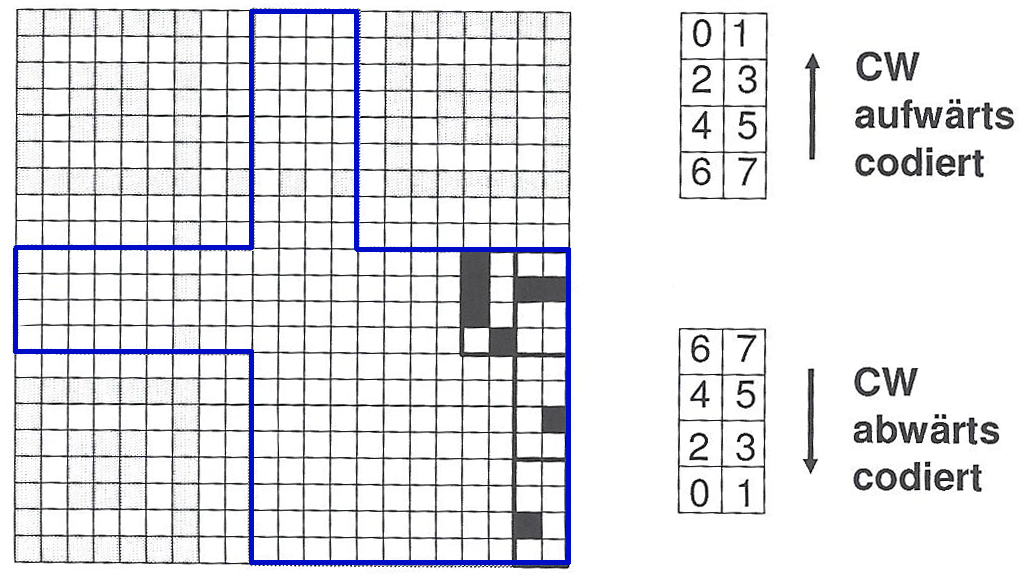
\includegraphics[width=8cm]{Bilder/QR_CW_einsetzen.png}
	\caption[4 Codewörter im Datenbereich]{4 Codewörter im Datenbereich\footnotemark}
	\label{fig:insertcw}
	\hfill
\end{figure}

\subsubsection*{6. Maskieren des Datenbereichs}
Im sechsten Schritt wird nun eine Maske über diesen Datenbereich der Matrix gelegt. Das heißt, sämtliche Bits werden mit einer vorgegebenen Maske ver-XOR-t. Insgesamt gibt es sieben Masken, die zuerst einmal alle auf die Matrix angewendet werden. Aus den daraus resultierenden sieben Codes wird derjenige bestimmt, der nach evaluieren vierer Eigenschaften mit Strafpunkten die wenigsten dieser Strafpunkte gesammelt hat. \\

Bei der Evaluierung geht es unter anderem darum, das Verhältnis von hellen zu dunklen Modulen insgesamt so ausgeglichen wie möglich zu halten und diese auch so gut wie möglich über den gesamten Code zu verteilen, sodass sich keine größeren dunklen und hellen Flecken bilden. 
Die verwendete Maske wird mit 3 Bit (000 bis 111)codiert, die im nächsten Schritt der Formatinformation hinzugefügt werden. 
\footnotetext{Quelle: \cite[204]{Lenk2012}}
Wer sich nun fragt, wie diese Maske denn für die verschiedenen Größen des QR-Codes aussieht, dem sei gesagt, dass sie sich per Algorithmus berechnen lassen.\footnote{siehe Abschnitt 8.8.1 des ISO-Standards 18004:2000} Abbildung~\ref{fig:qrmasks} zeigt die sieben Masken für einen QR-Code Version 1.
\begin{figure}[htbp]
	\centering
	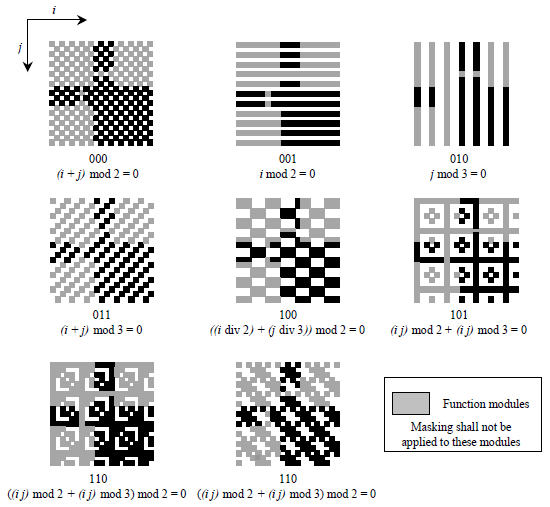
\includegraphics[width=12.7cm]{Bilder/QR_Mask_Patterns.png}
	\caption[Masken für einen QR-Code Version 1 inklusive ihrer Generatorfunktion]{Masken für einen QR-Code Version 1 inklusive ihrer Generatorfunktion\footnotemark}
	\label{fig:qrmasks}
	\hfill
\end{figure}
\footnotetext{Quelle: \cite[51]{ISO18004}}~

\subsubsection*{7. Format- und gegebenenfalls Versionsinformationen hinzufügen}
Nachdem alle Codewörter eingesetzt und maskiert wurden, werden im letzten Schritt noch die Formatinformationen hinzugefügt. Zu diesen zählen ein einzelnes schwarzes Modul, sowie 15 Bit Formatinformationen. Die ersten 5 Bit enthalten 2 Bit Fehlerkorrekturmodus (L = 01, M = 00, Q = 11, H = 10) und 3 Bit Maskennummer (siehe Schritt 6). Die restlichen 10 Bit dienen der Absicherung dieser ersten 5 Bit und werden nach BCH(15,5)\footnote{BCH steht für Bose-Chaudhuri-Hocquenghem-Codes. Diese sind zyklisch fehlerkorrigierende Codes, die u.a. in der Datenspeicherung verwendet werden. Näheres zu diesen Codes findet sich in der einschlägigen Literatur und soll nicht Teil dieser Arbeit sein.} ermittelt. Anschließend wird der 15 Bit String mit einer immer gleichen Maske (101010000010010) XOR maskiert.
Diese 15 maskierten Bits werden zwei mal in der Matrix eingesetzt: einmal links oben um das Suchmuster und einmal aufgeteilt unter dem Suchmuster rechts oben sowie rechts neben dem Suchmuster links unten (vgl. Abbildung~\ref{fig:formatinformationpositioning}).\\
\begin{figure}[htbp]
	\centering
	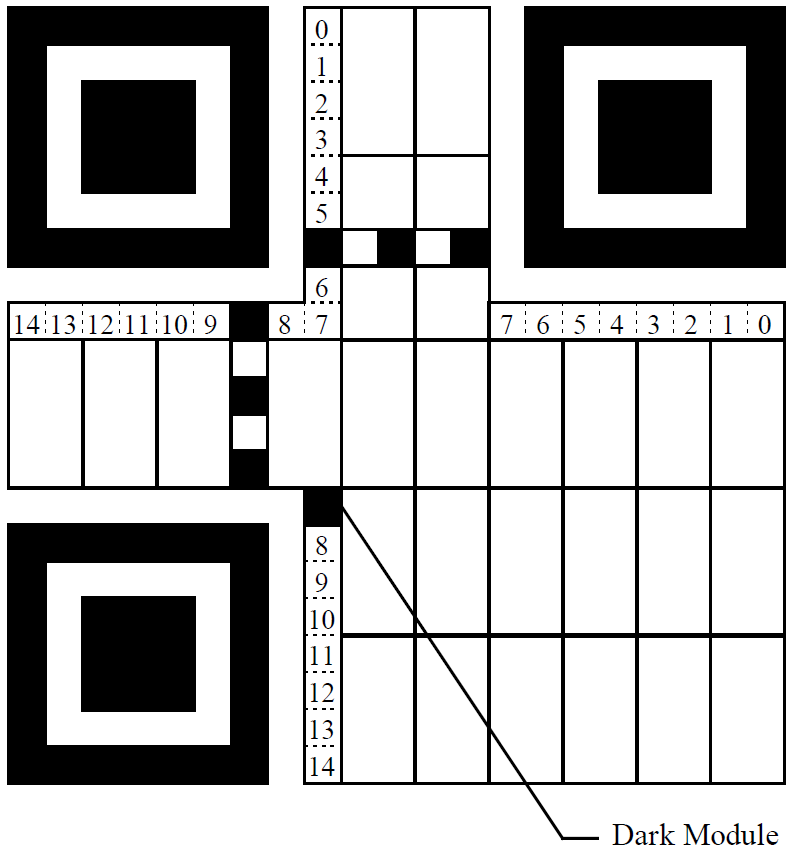
\includegraphics[width=9cm]{Bilder/QR_Format_Positioning.png}
	\caption[Positionieren der Formatinformationen]{Positionieren der Formatinformationen\footnotemark}
	\label{fig:formatinformationpositioning}
	\hfill
\end{figure}
~\\

Verwendet man einen QR-Code der Version 7 und höher, muss zusätzlich noch die Versionsnummer innerhalb der Matrix codiert werden. 
\footnotetext{Quelle: \cite[54]{ISO18004}}Sie wird in insgesamt 18 Bits codiert, von denen 6 Bits die Versionsnummer enthalten (z.B. 7 wird in 000111 codiert) und die restlichen 12 wieder der Fehlerkorrektion dienen und mit BCH(18,6) berechnet werden. Der resultierende Bit-String wird in diesem Fall nicht maskiert und nach Abbildung~\ref{fig:versioninformationpositioning} in einem 3 x 6 und einem 6 x 3 Modulblock positioniert.\\
%\vspace{-0.7cm}
\begin{figure}[htbp]
	\centering
	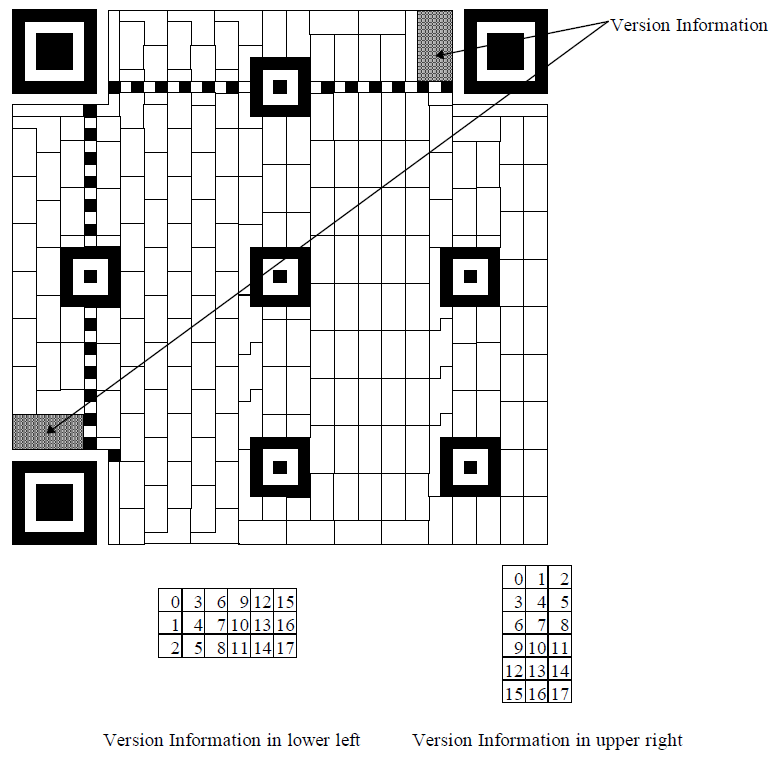
\includegraphics[width=15cm]{Bilder/QR_Version_Information.png}
	\caption[Positionieren der Versionsinformation]{Positionieren der Versionsinformation\footnotemark}
	\label{fig:versioninformationpositioning}
	\hfill
\end{figure}
\footnotetext{Quelle: \cite[55]{ISO18004}}~\\

Der nun fertige Code kann prinzipiell ausgedruckt oder auf einer Website platziert werden. Da er jedoch nach Spezifikation eine mindestens 4 Modulbreiten breite, umlaufende Ruhezone benötigt um sich für das schnelle und einfache Lesen von der Umgebung abzugrenzen, wird diese direkt in das resultierende Bild eingebaut. Somit wird gewährleistet, dass diese Mindestanforderung an die Ruhezone eingehalten wird.

\subsection{Exemplarisches Beispiel}
Um das im vorherigen Abschnitt beschriebene Vorgehen etwas konkreter darzustellen, soll in diesem Abschnitt die Ziffernfolge \glqq 01234567\grqq~exemplarisch in einen QR-Code der Version 1 mit dem Fehlerkorrekturmodus M umgesetzt werden. Das Beispiel wurde dem Buch \glqq QR-Code\grqq~von Bernhard Lenk (\cite{Lenk2012}), Kapitel 10.1 entnommen.

\textbf{1. Datenanalyse:}\\
Da das Beispiel eine reine Ziffernfolge codieren soll, wird der Numerik-Modus gewählt. Da insgesamt nur acht Stellen codiert werden müssen, reicht der kleinste QR-Code (Version 1) aus. Dieser kann je nach Fehlerkorrekturstufe (FKS) 17 bis 41 Ziffern aufnehmen. Als FKS wurde M gewählt. Aus diesen Voraussetzungen ergibt sich, dass der QR-Code am Ende 26 Codeworte in seinem Datensegment enthält: 16 DCW und 10 FKCW. 

\textbf{2. In Bitstring umwandeln, auffüllen und splitten:}\\
Zuerst wird nun die Ziffernfolge in Tripel aufgeteilt: 012 345 67 ($\rightarrow$ es ergibt sich ein Rest von 2 Stellen).\\
Die Tripel werden nun in 8 Bit gewandelt, das restliche Paar nur in 7: \\
\centerline{$012_{10}~\rightarrow~0000001100_2$}
\centerline{$345_{10}~\rightarrow~0101011001_2$}
\centerline{$~67_{10}~\rightarrow~~~~1000011_2$}\\
Nun wird noch die Anzahl der Stellen (8) nach Tabelle~\ref{tab:encodenumberofcharacters} in 10 Bit gewandelt:~\\
\centerline{$8_{10}~\rightarrow~0000001000_2$}\\
Verkettet man nun Betriebsmodus (Numerik), Stellenzahl, die binären Nutzdaten und den Terminator, ergibt sich folgender Datenstring:~\\
\centerline{$0001~~0000001000~~000001100~0101011001~1000011~~0000$}\\
Da bereits festgestellt wurde, dass der QR-Code 16 DCW enthält, muss dieser Datenstring nun in 8er-Blöcke aufgeteilt und auf 16 DCW aufgefüllt werden:\\
Gruppieren:\\
\centerline{$00010000~00100000~00001100~01010110~01100001~10000$}\\
plus 000 zum Auffüllen auf 8 Bit:\\
\centerline{$00010000~00100000~00001100~01010110~01100001~10000000$}\\

Somit ergeben sich 6 DCW. Da wir aber 16 DCW belegen müssen, werden einfach abwechselnd die beiden FCW 11101100 und 00010001 hinzugefügt (Zeile 2 und 3):~\\
\centerline{$00010000~00100000~00001100~01010110~01100001~10000000$}
\centerline{$11101100~00010001~11101100~00010001~11101100~00010001$}
\centerline{$11101100~00010001~11101100~00010001~~~~~~~~~~~~~~~~~~~~~~~~~~$}
 
\textbf{3. FKCW nach Reed-Solomon berechnen und umwandeln:}\\
Das Ergebnis der Polynomrechnung sieht folgendermaßen aus:\hfill ~\\
\centerline{$10100101~00100100~11010100~11000001~11101101~00110110$}
\centerline{$11000111~10000111~00101100~01010101~~~~~~~~~~~~~~~~~~~~~~~~~~$}

\textbf{4. Verschränken der DCW und der FKCW:}\\
Nun da die Daten als Bit-String vorliegen und aufgefüllt wurden und auch die FKCW nach Reed-Solomon bestimmt wurden, werden nun beide Bit-Strings einfach hintereinander gehängt:\\
CW 1\\
\centerline{$00010000~00100000~00001100~01010110~01100001~10000000$}
\centerline{$11101100~00010001~11101100~00010001~11101100~00010001$}
\centerline{$11101100~00010001~11101100~00010001~10100101~00100100$}
\centerline{$11010100~11000001~11101101~00110110~11000111~10000111$}
\centerline{$00101100~01010101~~~~~~~~~~~~~~~~~~~~~~~~~~~~~~~~~~~~~~~~~~~~~~~~~~~~$}
bis CW 26

\textbf{5. Einsetzen der Codewörter in die Matrix}\\
Wie in Abbildung~\ref{fig:filldata} dargestellt, werden dann die Daten als Blöcke einfach beginnend rechts unten und dann im Zick-Zack (den Pfeilen folgend) nach links in die Matrix gefüllt. Die Blöcke kommen dabei direkt nacheinander und werden nur an den blau markierten Stellen durch die Taktzellen unterbrochen. Die rechte der beiden Matrix-Abbildungen zeigt die mit Daten gefüllte Matrix.
\begin{figure}[htbp]
	\parbox{.47\textwidth}
	{
		\centering
		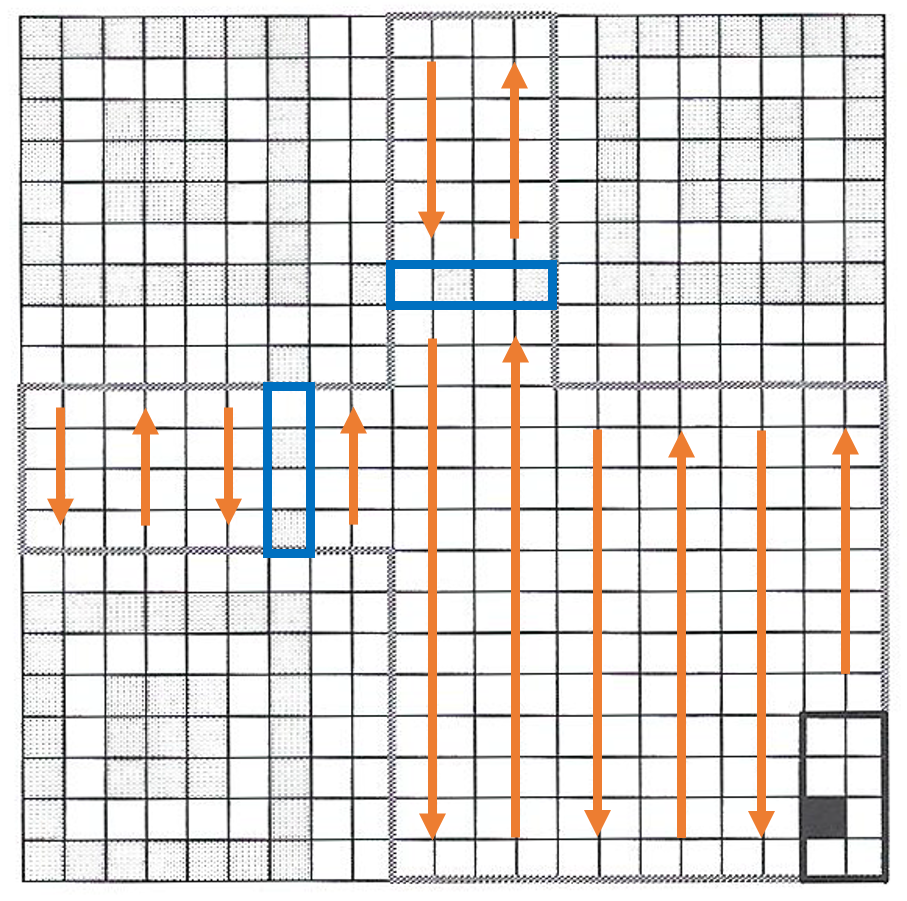
\includegraphics[height=4.8cm]{Bilder/QR_Fill_Data_Start_1.png}
	}
	\hfill
	\parbox{.47\textwidth}
	{
		\centering
		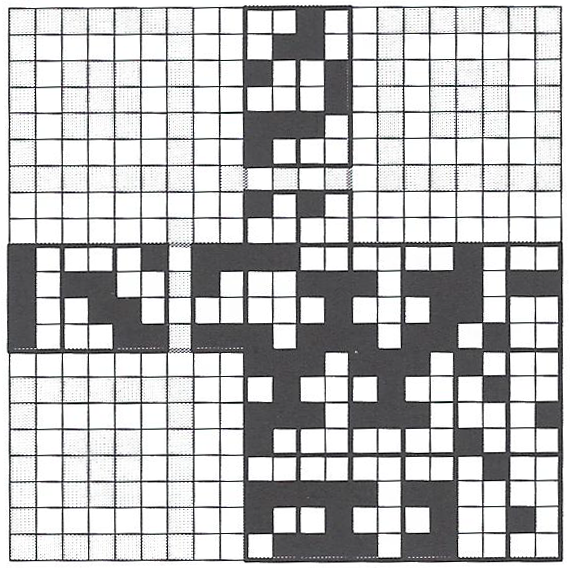
\includegraphics[height=4.8cm]{Bilder/QR_Fill_Data_End.png}
		%\caption[Drehwinkel]{Drehwinkel\textsuperscript{\ref{ftn:first}}}
		%\label{fig:drehwinkel}
	}
\caption[Füllen der Matrix mit Daten]{Füllen der Matrix mit Daten\footnotemark}
\label{fig:filldata}
	\hfill
\end{figure}
~\\

\textbf{6. Maskieren des Datenbereichs:}\\
Nun wird der Datenbereich mit allen Masken maskiert und evaluiert, welche die geringste Anzahl an Strafpunkten verursacht. Im vorliegenden Fall ist das die Maske 2, die mit 010 codiert wird.

\textbf{7. Formatinformationen hinzufügen:}
Im letzten Schritt werden dann die Formatinformationen gesammelt, codiert und zusammen mit den 
Suchmustern, den Taktzellen und dem fixen dunklen Modul eingesetzt.

Die 15 Bit Formatinformation werden wie folgt zusammengesetzt:\\
2 Bit Fehlerkorrekturmodus $\rightarrow$ hier M $\rightarrow$ 00 \\
3 Bit Maske  $\rightarrow$ hier Maske 2  $\rightarrow$ 010 \\
Die restlichen 10 Bit zur Fehlerkorrektur dieser Formatinformationen werden nach BCH(15,5) ermittelt und lauten im vorliegenden Beispiel 1001101110.\footnotetext{Quelle: \cite[201,216]{Lenk2012}}
Somit ergibt sich der 15 Bit-String 000101001101110.\\
Dieser wird anschließend noch mit der Maske 101010000010010 ver-XOR-t:\\
\centerline{XOR: 000101001101110}
\centerline{~~~~~~~~~101010000010010}
\centerline{$\rightarrow$~~~~~~101111001111100}\\
Mit der abschließend hinzugefügten Ruhezone ist der Code nun fertig aufgebaut (siehe Abbildung~\ref{fig:qrexamplefinal}).
\begin{figure}[htbp]
	\centering
	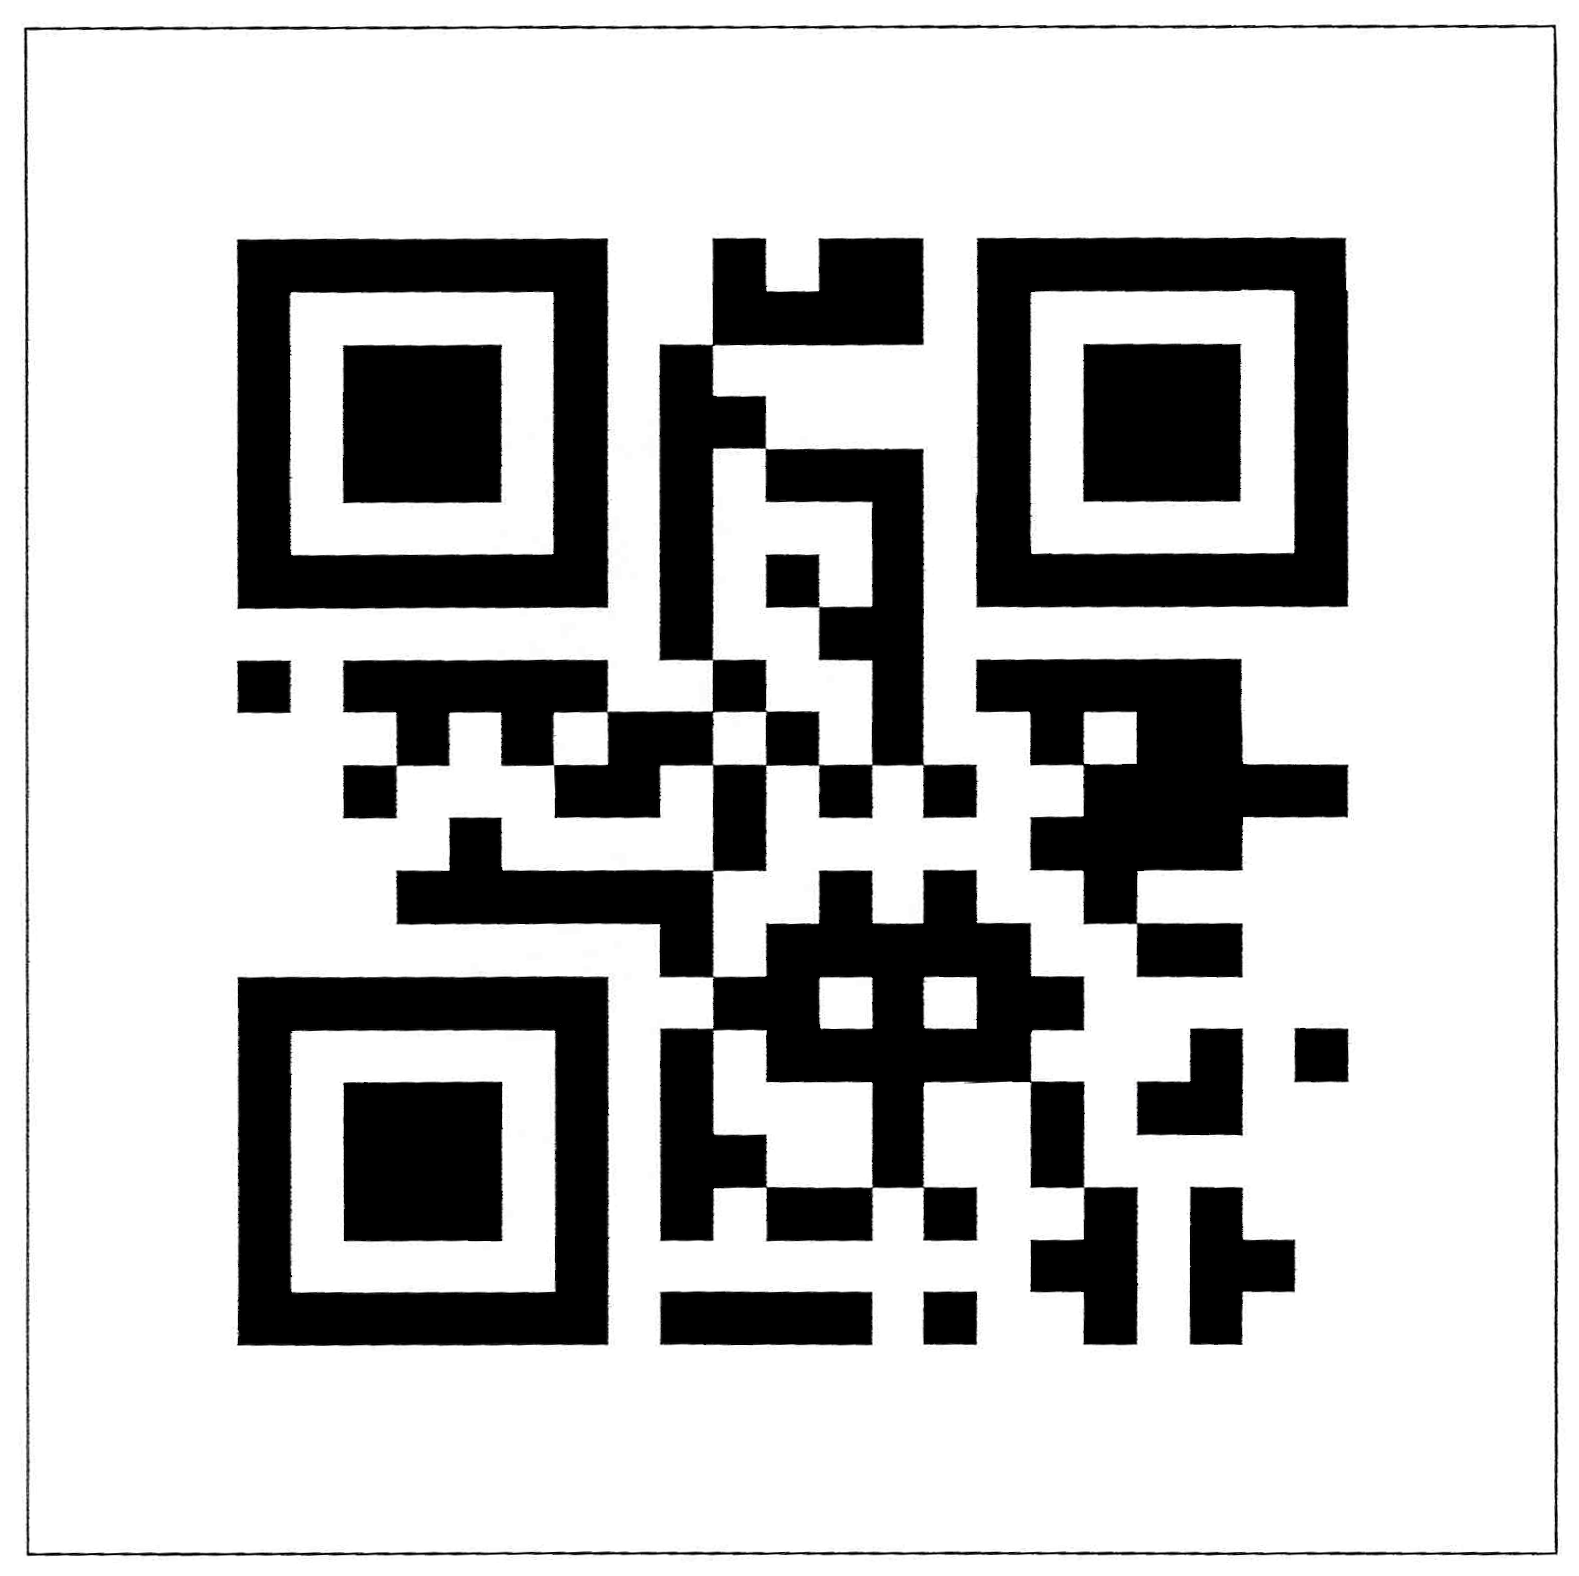
\includegraphics[width=5cm]{Bilder/QR_Example_Final.png}
	\caption[Fertiger QR-Code mit den Nutzdaten 01234567]{Fertiger QR-Code mit den Nutzdaten 01234567\footnotemark}
	\label{fig:qrexamplefinal}
\end{figure}
\footnotetext{Quelle: \cite[226]{Lenk2012}}~\pagebreak

\subsection{Daten lesen}
Besitzt man das Wissen, wie ein QR-Code aufgebaut ist und sein Inhalt codiert wird, so ist es eine recht einfache Übung, dieses Wissen in umgekehrter Reihenfolge anzuwenden und so einen gegebenen QR-Code zu decodieren.\\
Zu Beginn des Vorgangs muss zuerst einmal ermittelt werden, wie groß der gegebene Code ist und somit, von welcher Version er ist. Diese Information kann anhand des Abstandes zwischen den Suchmustern sowie mithilfe der Taktzellen recht einfach festgestellt werden.\\
Im nächsten Schritt wird der Formatinformations-Bit-String ausgelesen und mit der Maske 101010000010010 und XOR demaskiert. So erhält man den Fehlerkorrekturmodus und die Nummer der Maske, welche zur Maskierung der Daten benutzt wurde.\\
Diese muss wieder mit Hilfe von XOR von den Daten entfernt werden, um an die realen Datenbits zu kommen.\\
Aus der Versionsnummer ist nun ersichtlich, wie viele Codewörter im Datenbereich insgesamt vorhanden sind. Durch den Fehlerkorrekturmodus ist auch bekannt, wie viele davon FKCW sind und wie viele reine DCW.\\
Die CW werden nun wieder von rechts unten aus Block für Block ausgelesen und zu dem langen Bit-String zusammengesetzt. Der aufmerksame Leser wird sich noch erinnern, dass die ersten 4 Bit von links des langen Strings die Information über den verwendeten Betriebsmodus des QR-Codes enthalten.\\
Wenn der Modus bekannt ist, ist auch bekannt, wie viele der darauf folgenden Bit die Anzahl der codierten Zeichen repräsentieren (siehe Tabelle~\ref{tab:encodenumberofcharacters}). Nun werden die Bits bis zum Auftauchen des Terminators in Blöcke entsprechend dem Modus geteilt und aus dem Binärformat zurück ins ursprünglich verwendete Format gewandelt.
     
\pagebreak
